\documentclass{article}
%\usepackage{vcbm2016}

% --- for  Annual CONFERENCE
% \ConferenceSubmission % uncomment for Conference submission
% \ConferencePaper      % uncomment for (final) Conference Paper
% \STAR                 % uncomment for STAR contribution
% \Tutorial             % uncomment for Tutorial contribution
% \ShortPresentation    % uncomment for (final) Short Conference Presentation
%
% --- for  CGF Journal
% \JournalSubmission    % uncomment for submission to Computer Graphics Forum
% \JournalPaper         % uncomment for final version of Journal Paper
%
% --- for  EG Workshop Proceedings
%\WsSubmission    % uncomment for submission to EG Workshop
% \WsPaper         % uncomment for final version of EG Workshop contribution
%
%\electronicVersion % can be used both for the printed and electronic version

% !! *please* don't change anything above
% !! unless you REALLY know what you are doing
% ------------------------------------------------------------------------

% for including postscript figures
% mind: package option 'draft' will replace PS figure by a filname within a frame
%\ifpdf \usepackage[pdftex]{graphicx} \pdfcompresslevel=9
%\else \usepackage[dvips]{graphicx} \fi

%\PrintedOrElectronic

% prepare for electronic version of your document
\usepackage{t1enc,dfadobe}
\usepackage{graphicx}




\begin{document}
	\begin{figure}[t]
		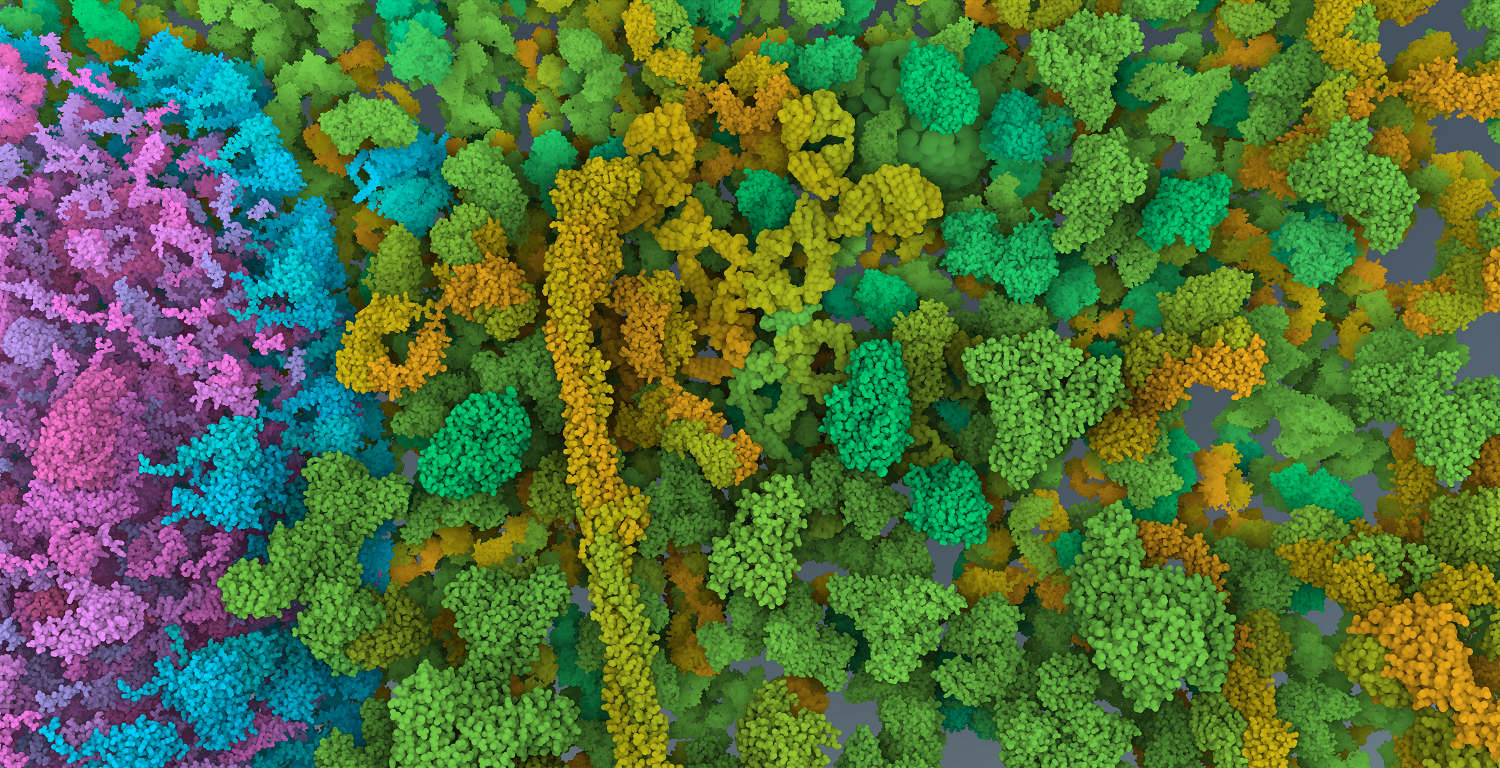
\includegraphics[width=0.95\linewidth,keepaspectratio]{supplementaryMaterial/domain60} 
		
		\vspace{0.1cm}
		
		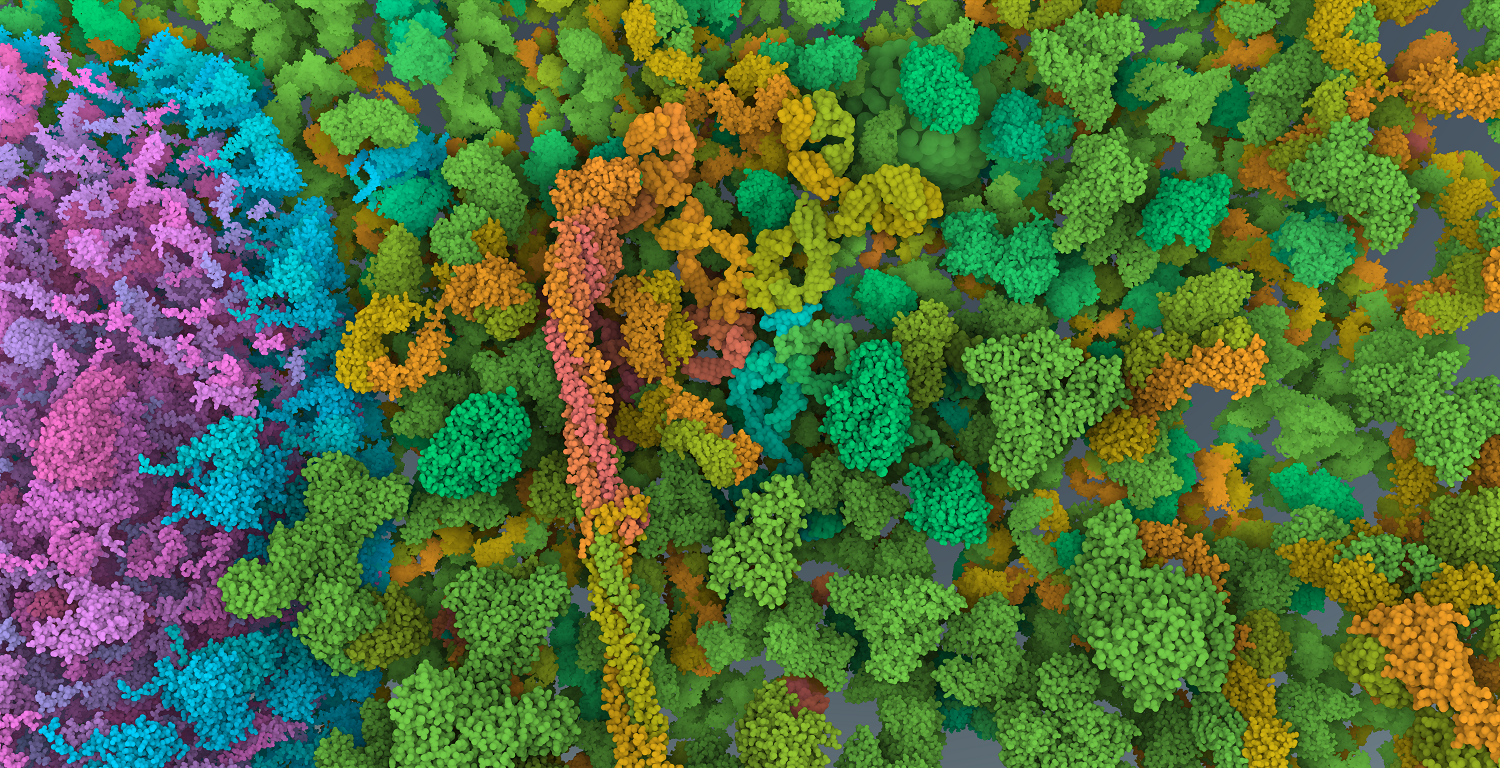
\includegraphics[width=0.95\linewidth,keepaspectratio]{supplementaryMaterial/domain180} 
		
		\vspace{0.1cm}
		
		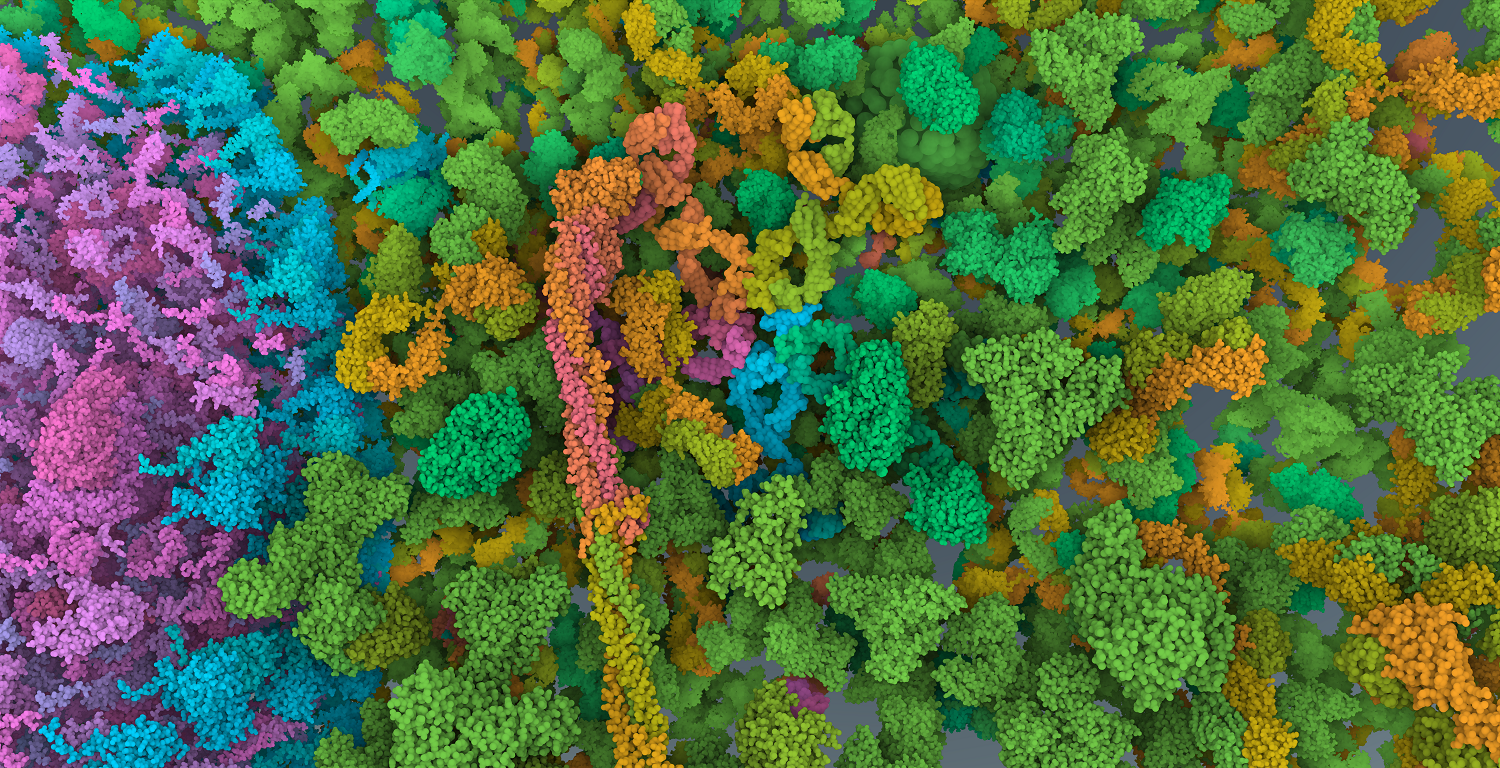
\includegraphics[width=0.95\linewidth,keepaspectratio]{supplementaryMaterial/domain300} 
		\caption{Wedges for domain angle values set to 60 (top), 180 (middle), and 300 (bottom) degrees. Important are the rod like protein in the foreground and the more partially blue protein in the background.}
	\end{figure}
	
	\begin{figure}[t]
		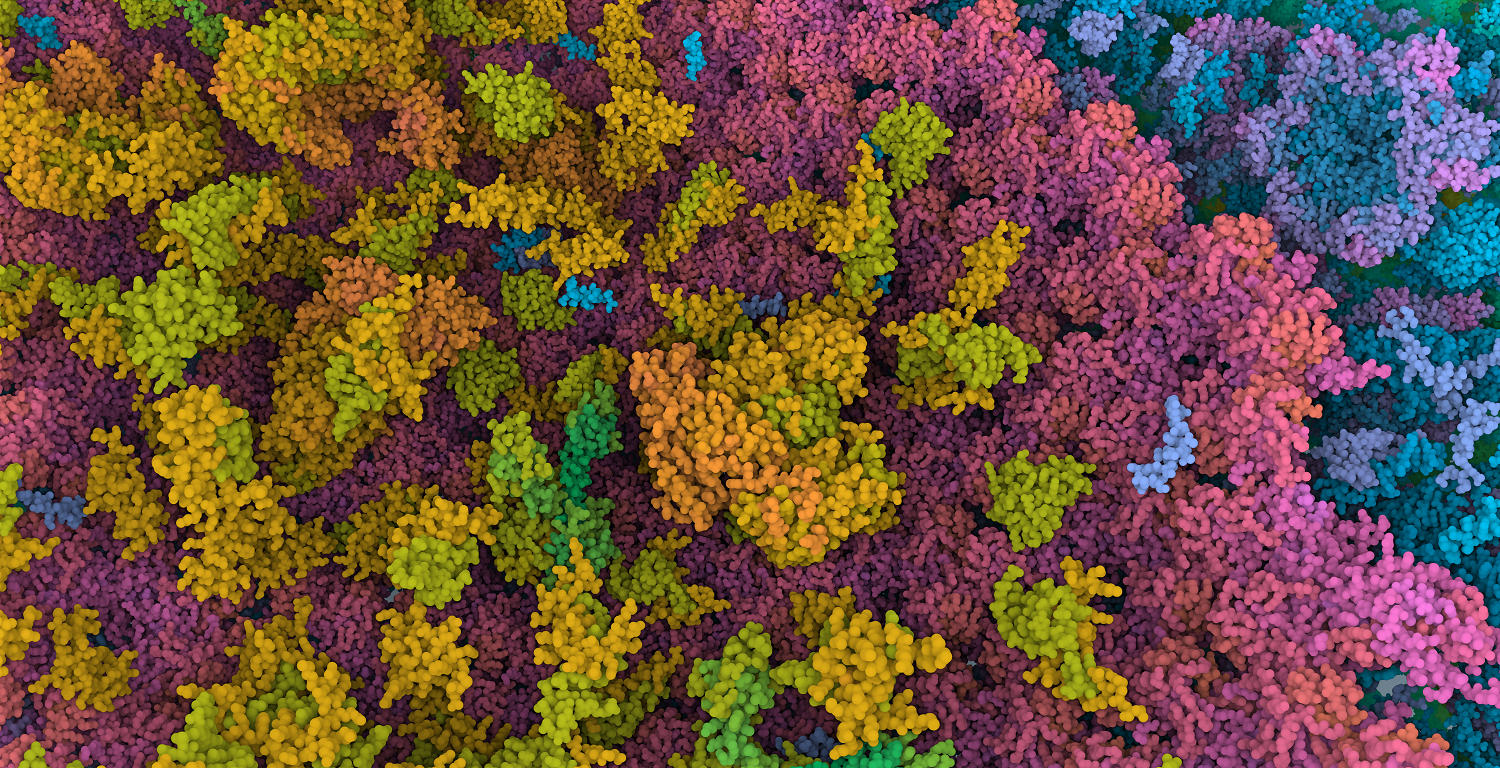
\includegraphics[width=0.95\linewidth,keepaspectratio]{supplementaryMaterial/secondary60} 
		
		\vspace{0.1cm}
		
		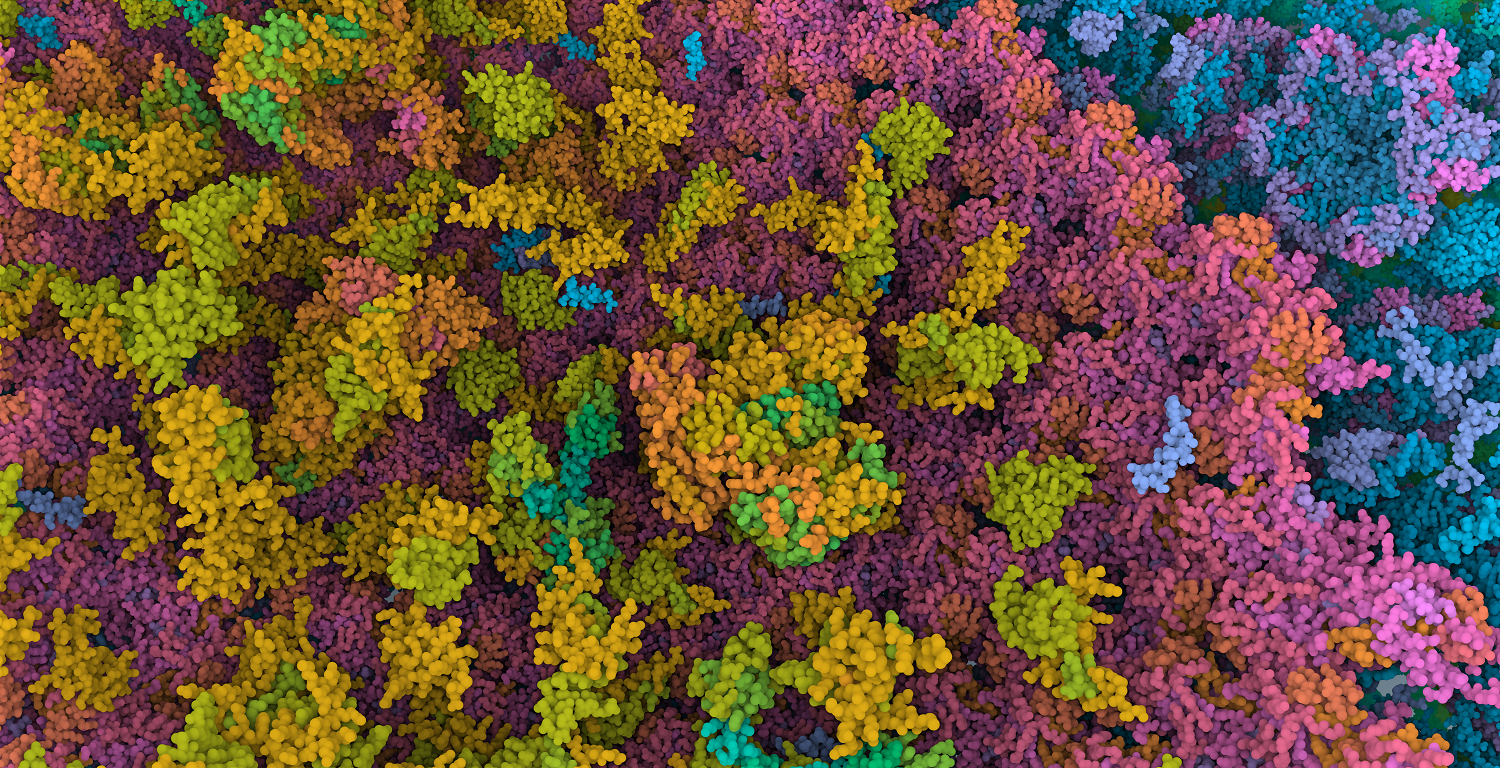
\includegraphics[width=0.95\linewidth,keepaspectratio]{supplementaryMaterial/secondary180} 
		
		\vspace{0.1cm}
		
		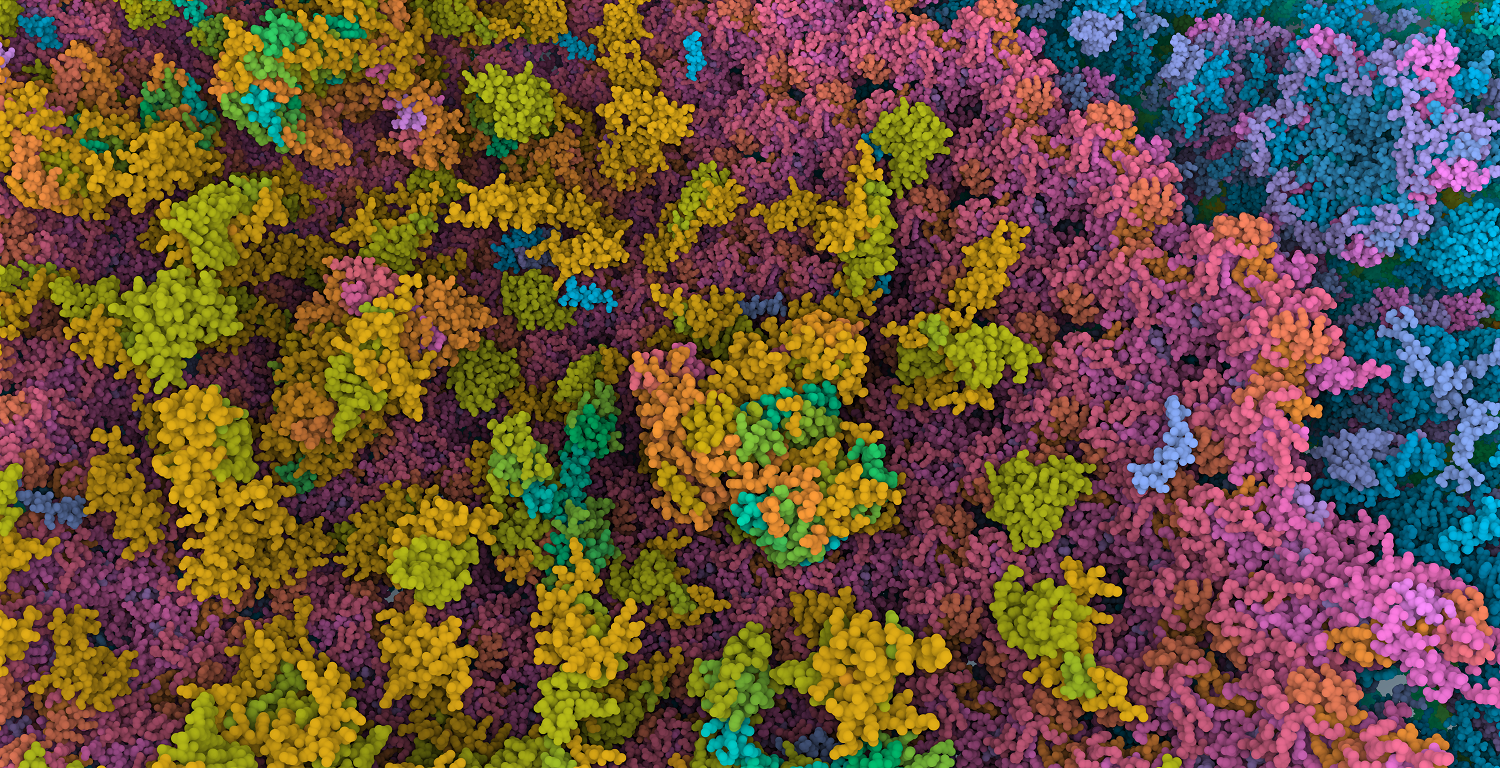
\includegraphics[width=0.95\linewidth,keepaspectratio]{supplementaryMaterial/secondary300} 
		\caption{Wedges for secondary structure angle values set to 60 (top), 180 (middle) and 300 (bottom) degrees. Important are the rod like protein in the foreground and the more partially blue protein in the background. Domain angles were kept at maximum 180 degrees.}
	\end{figure}
	
	
	\begin{figure}[t]
		\centering
		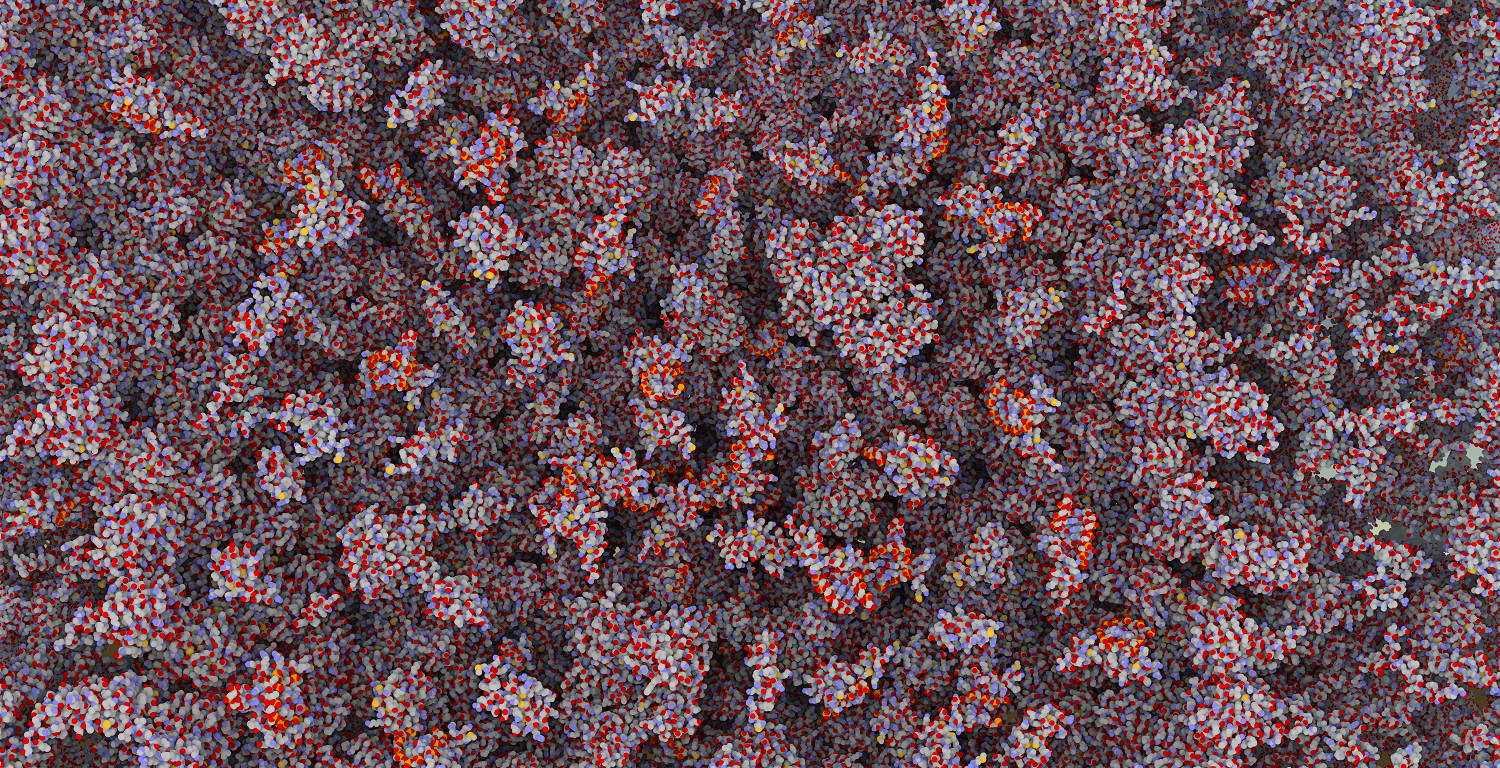
\includegraphics[width=0.95\linewidth,keepaspectratio]{supplementaryMaterial/atomzoomedin} 
		
		\vspace{0.1cm}
		
		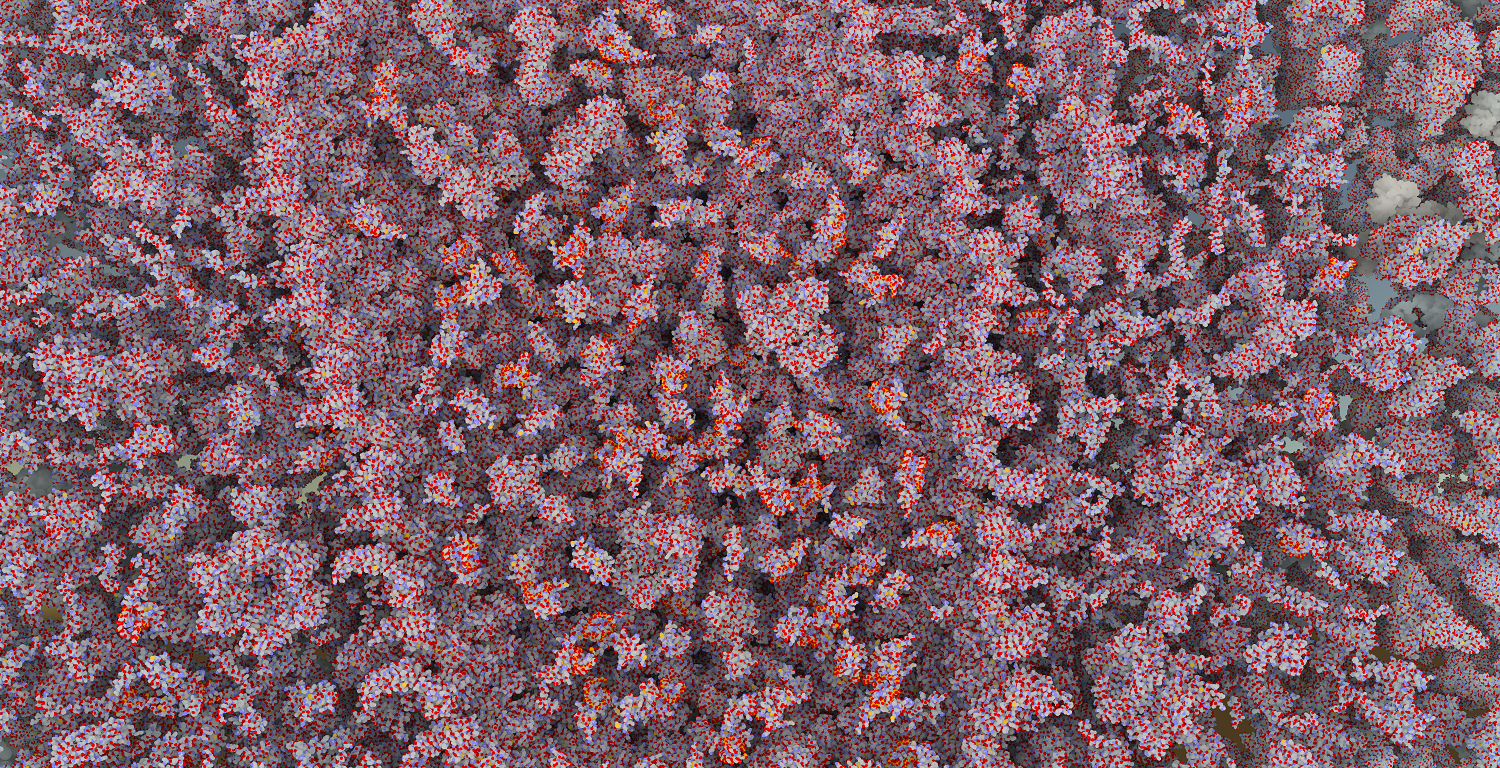
\includegraphics[width=0.95\linewidth,keepaspectratio]{supplementaryMaterial/atomzoomedmiddle} 
		
		\vspace{0.1cm}
		
		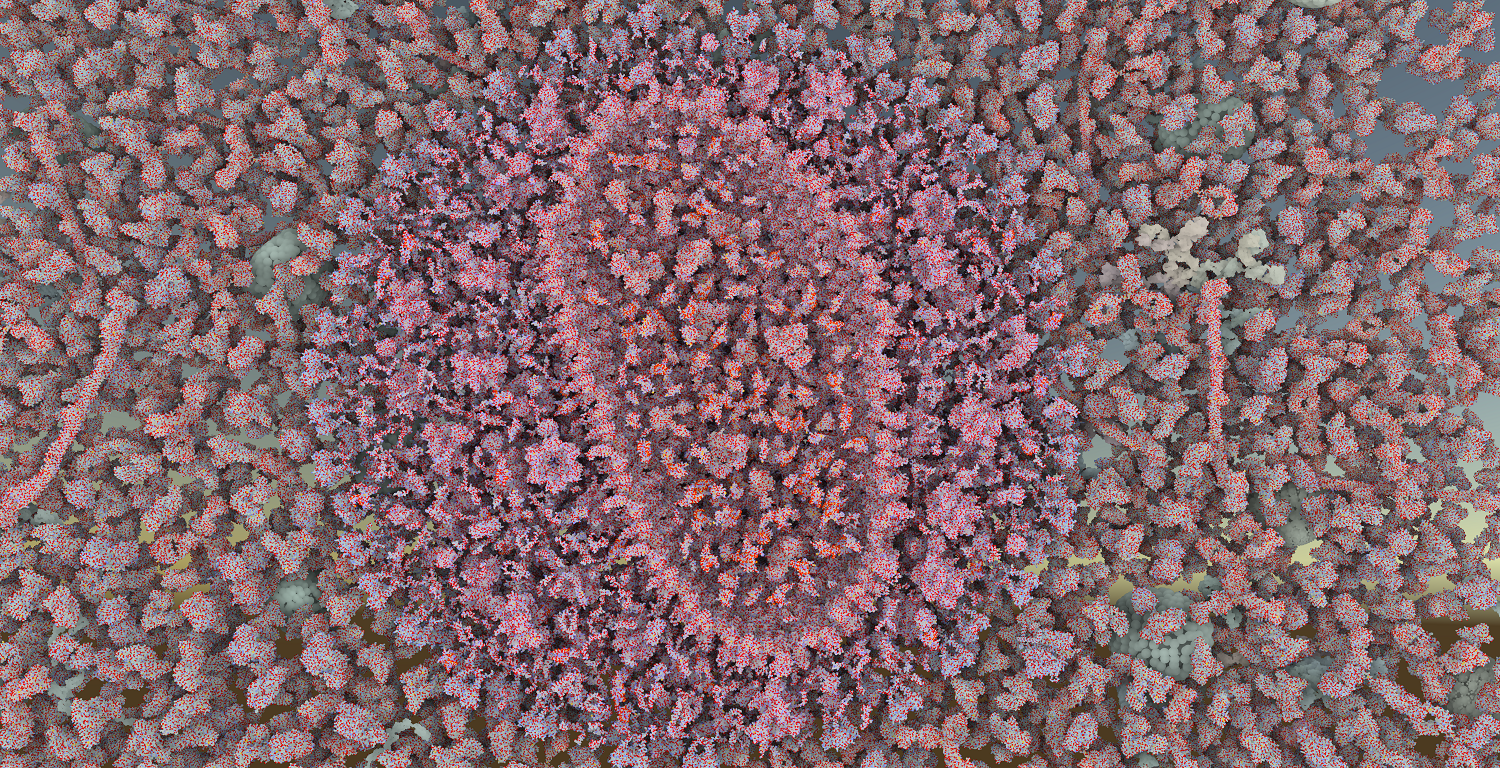
\includegraphics[width=0.9\linewidth,keepaspectratio]{supplementaryMaterial/atomzoomedhiv} 
		\caption{display of visualization using only colors for atoms at different zoom levels.}
	\end{figure}
	
	\begin{figure}[t]
		\centering
		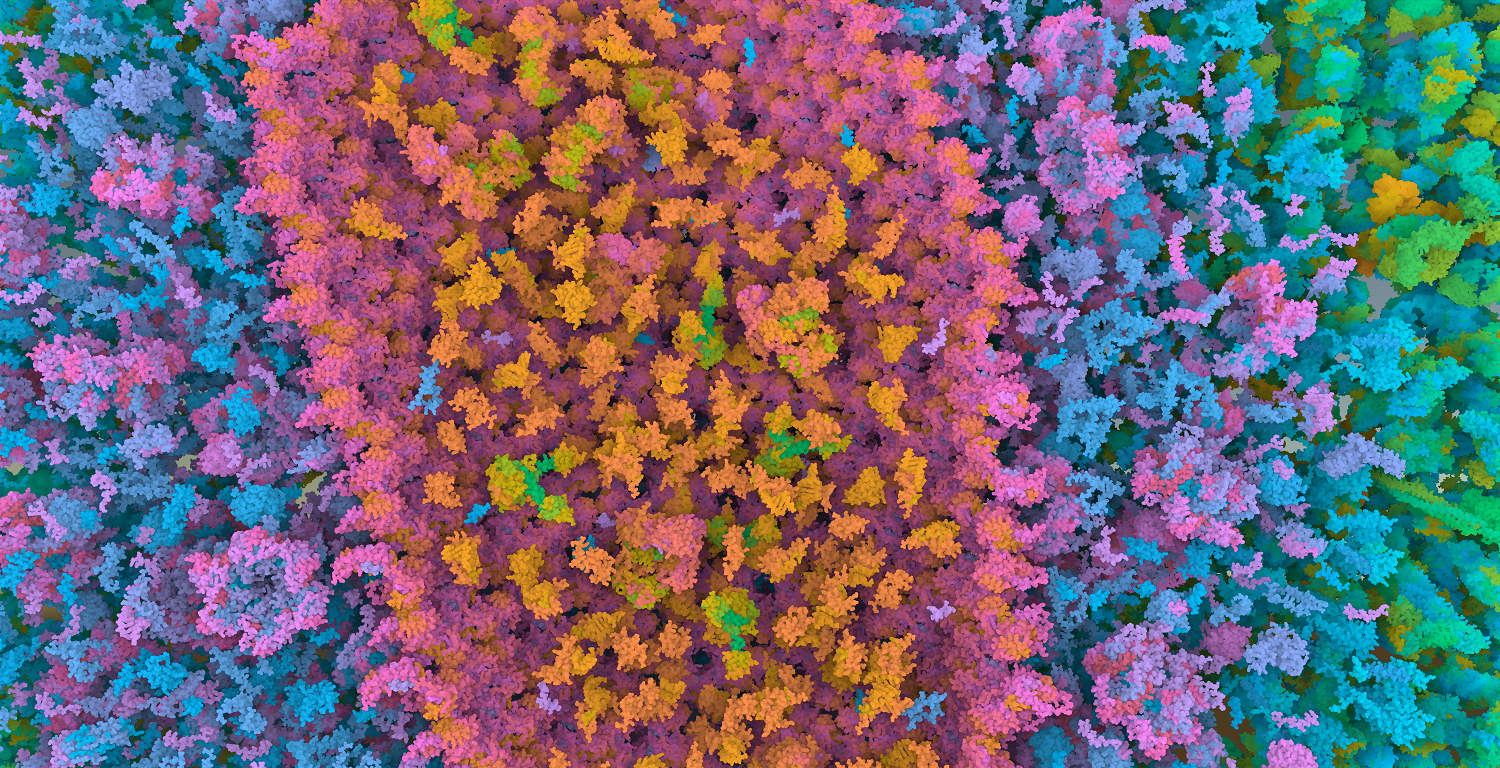
\includegraphics[width=0.95\linewidth,keepaspectratio]{supplementaryMaterial/secondaryzoomedmiddle} 
		
		\vspace{0.1cm}
		
		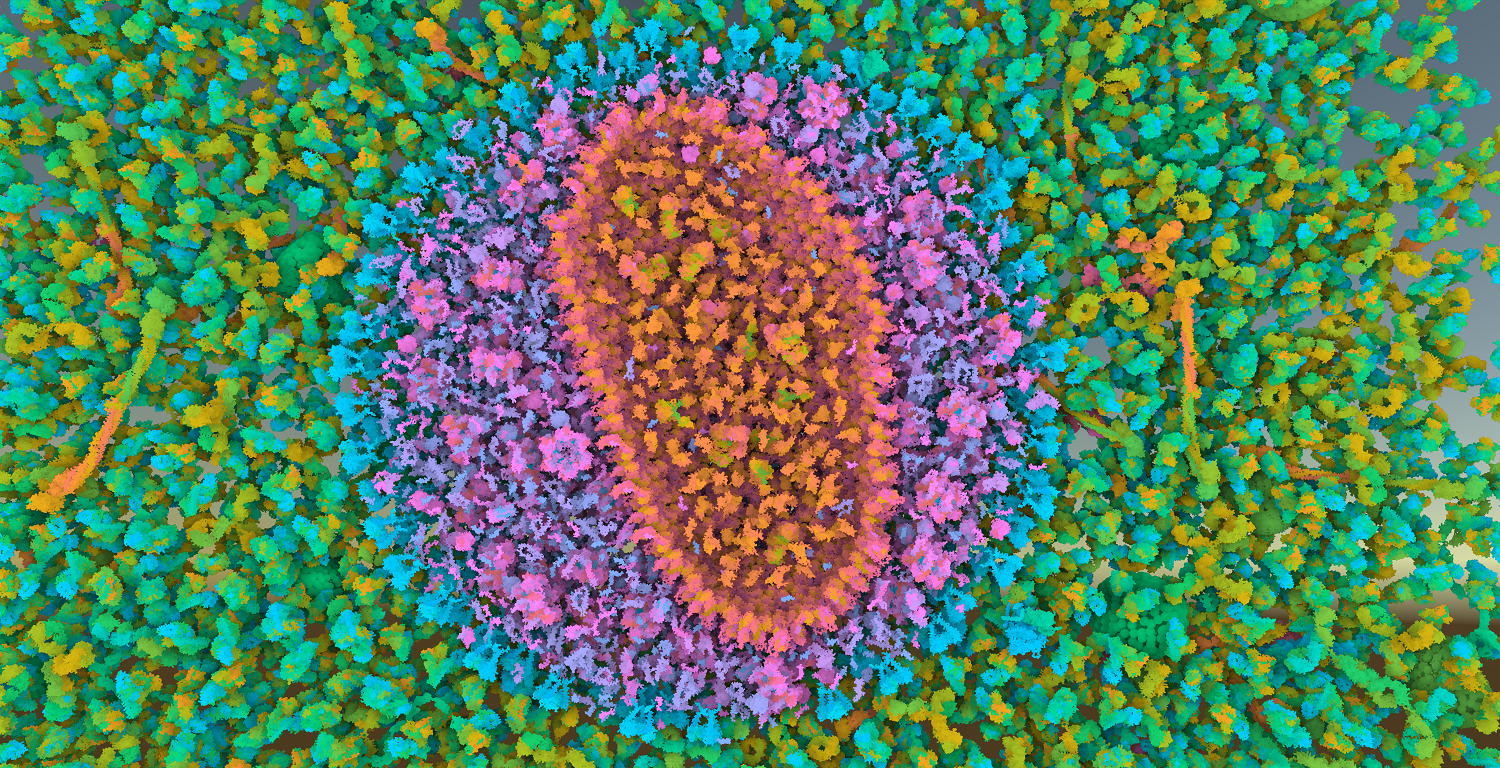
\includegraphics[width=0.95\linewidth,keepaspectratio]{supplementaryMaterial/secondaryzoomedhiv} 
		
		\vspace{0.1cm}
		
		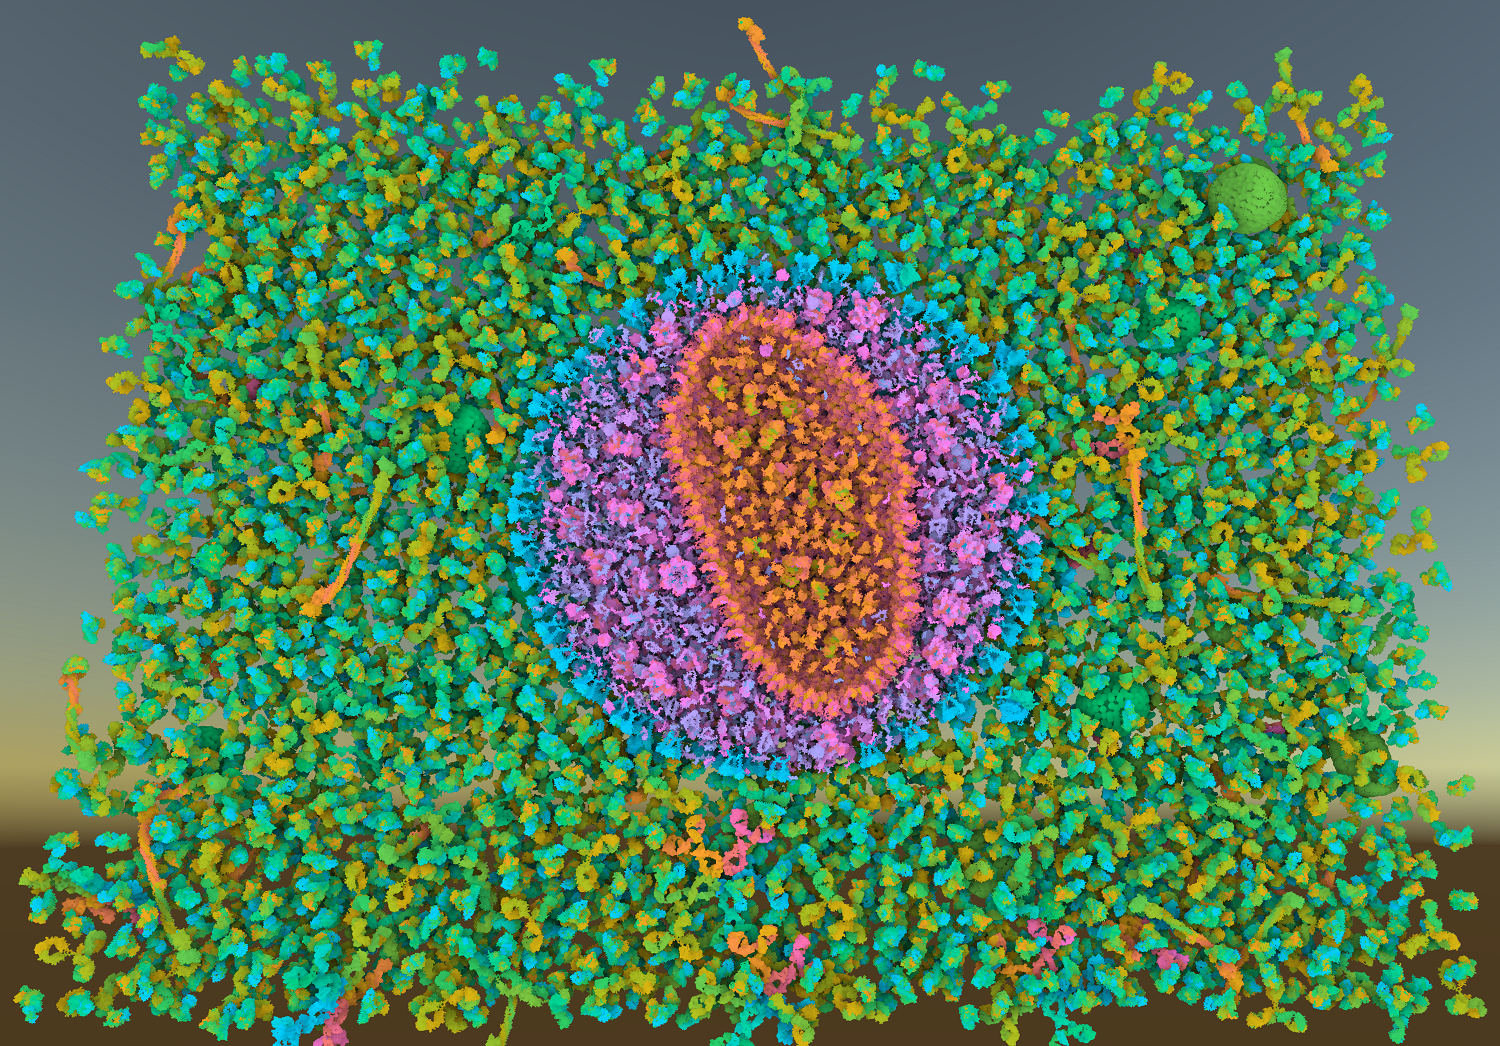
\includegraphics[width=0.8\linewidth,keepaspectratio]{supplementaryMaterial/secondaryzoomedfull} 
		\caption{display of visualization using only secondary structure colors at different zoom levels.}
	\end{figure}
	
	
	
	\begin{figure}[t]
		\centering
		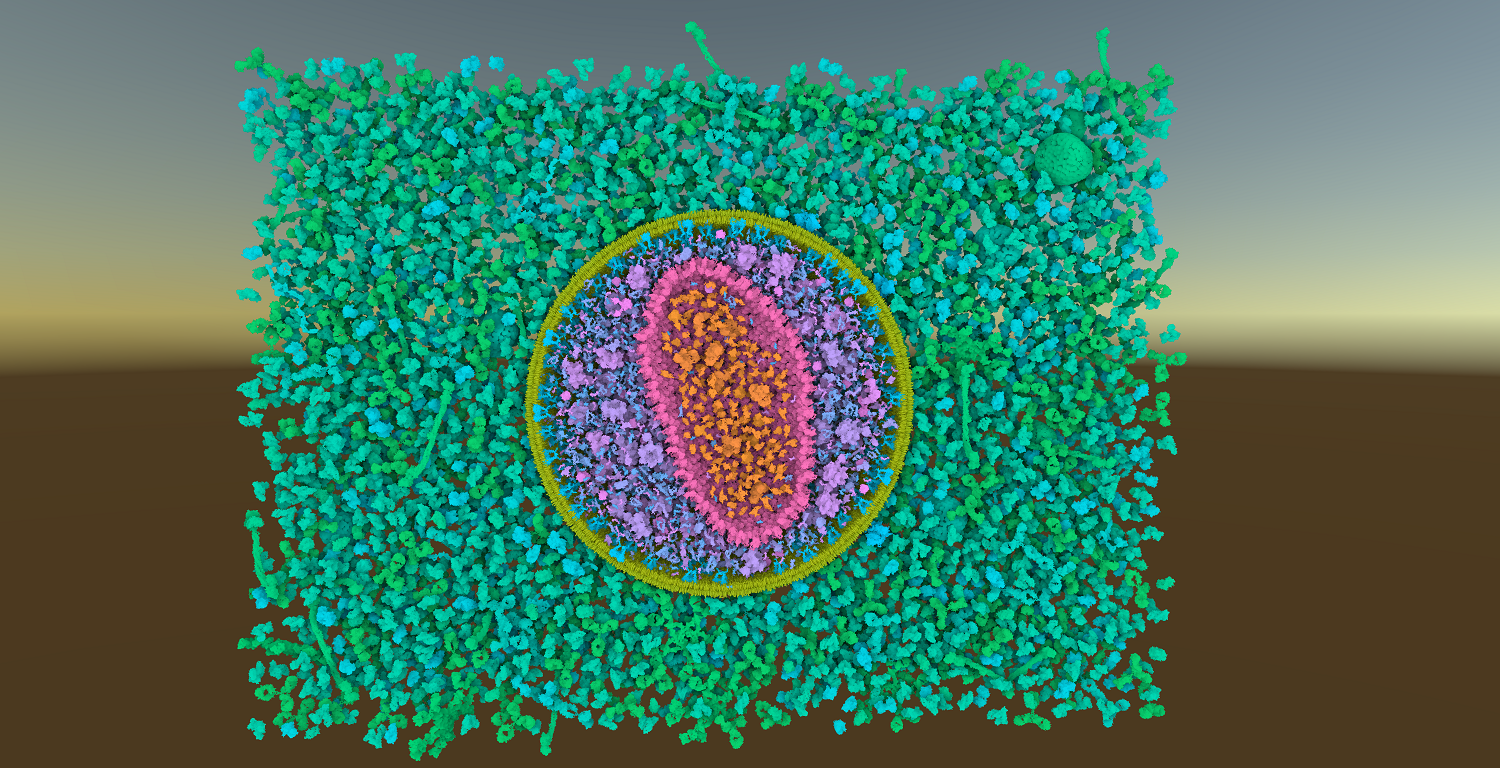
\includegraphics[width=0.95\linewidth,keepaspectratio]{supplementaryMaterial/userfull} 
		
		\vspace{0.1cm}
		
		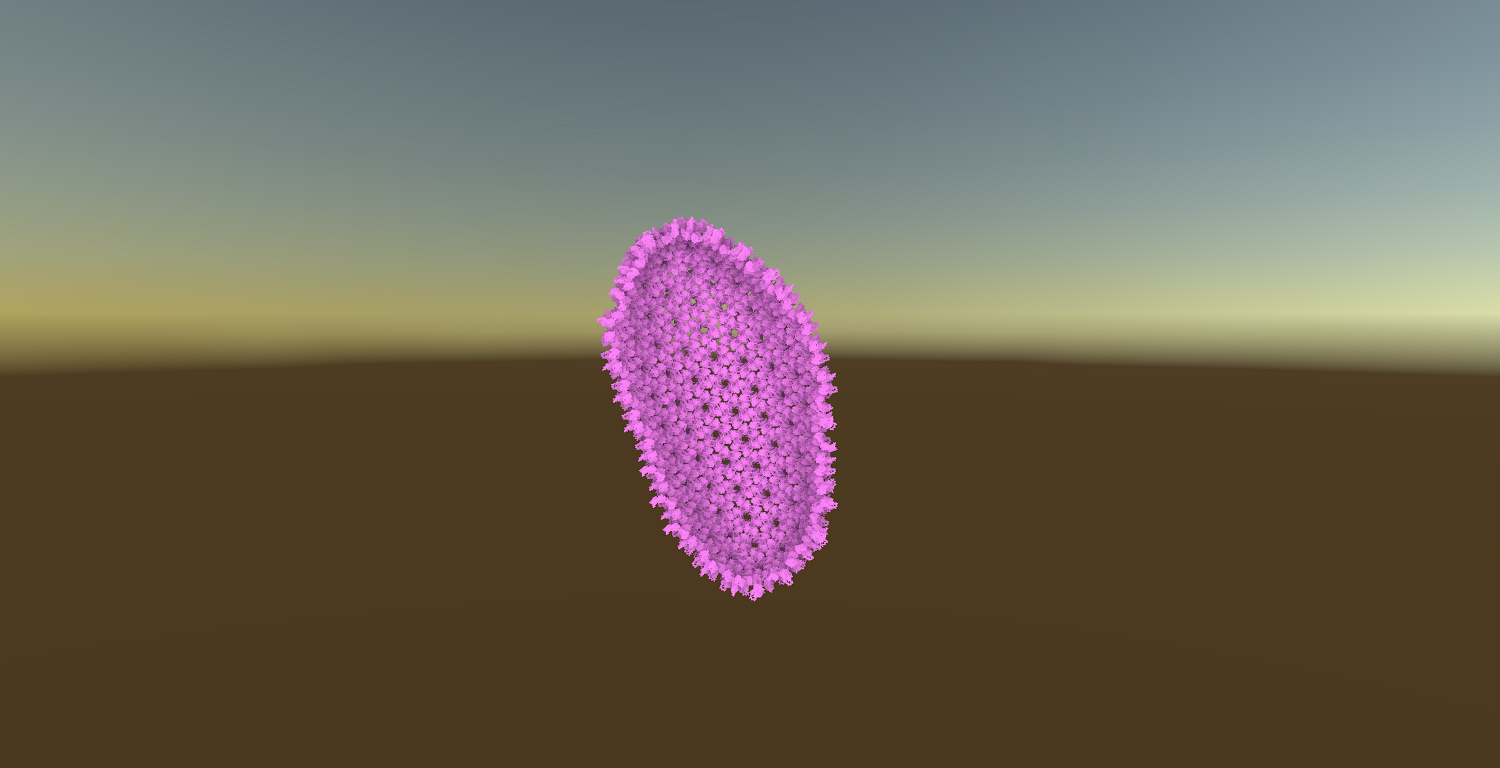
\includegraphics[width=0.95\linewidth,keepaspectratio]{supplementaryMaterial/usercapsid} 
		
		\vspace{0.1cm}
		
		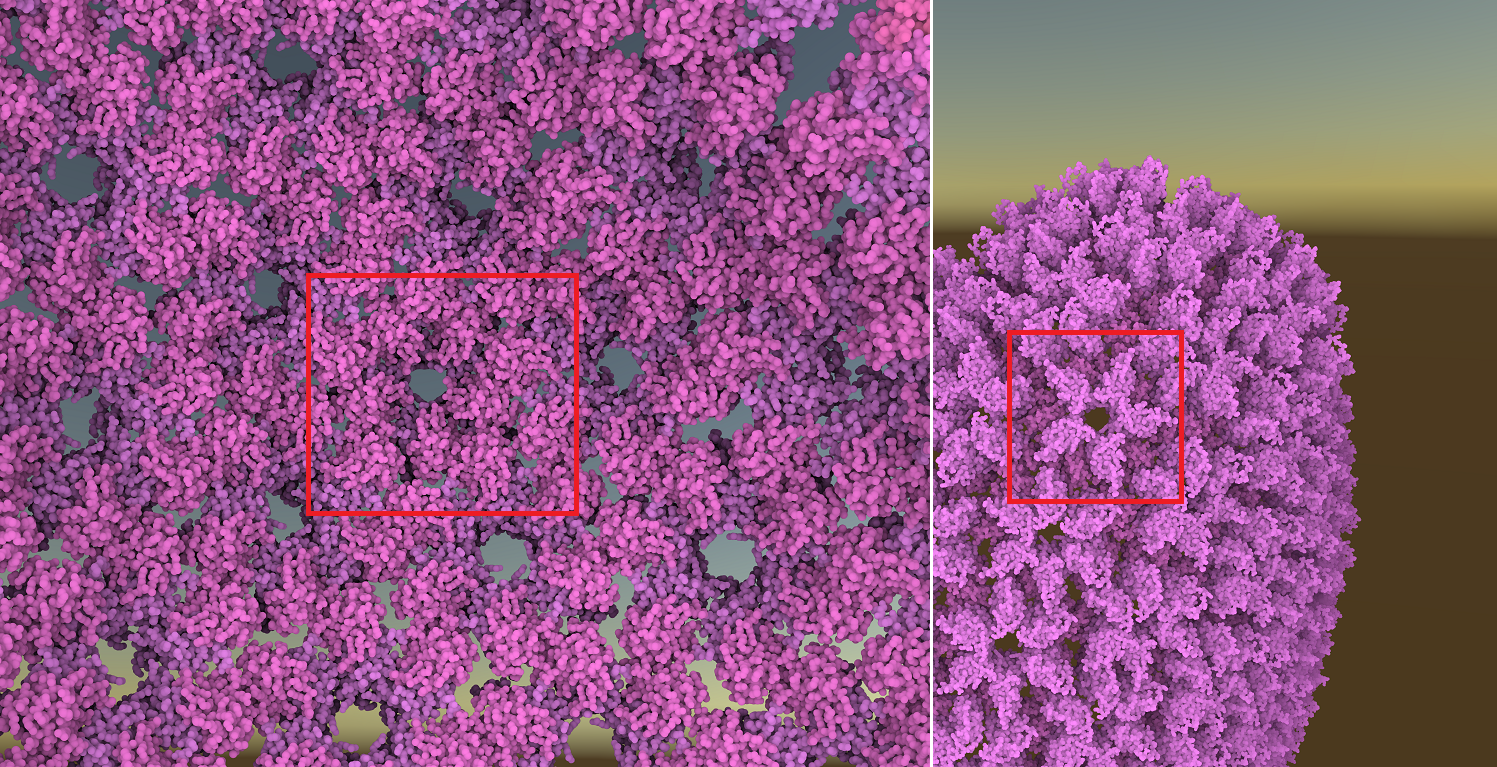
\includegraphics[width=0.95\linewidth,keepaspectratio]{supplementaryMaterial/bothpentamer} 
		\caption{User study search task. Top: complete visualization. Middle: capsid only. Bottom: pentamer, from interior (left) and exterior (right), in red box.}
	\end{figure}
	
	\begin{figure}[t]
		\centering
		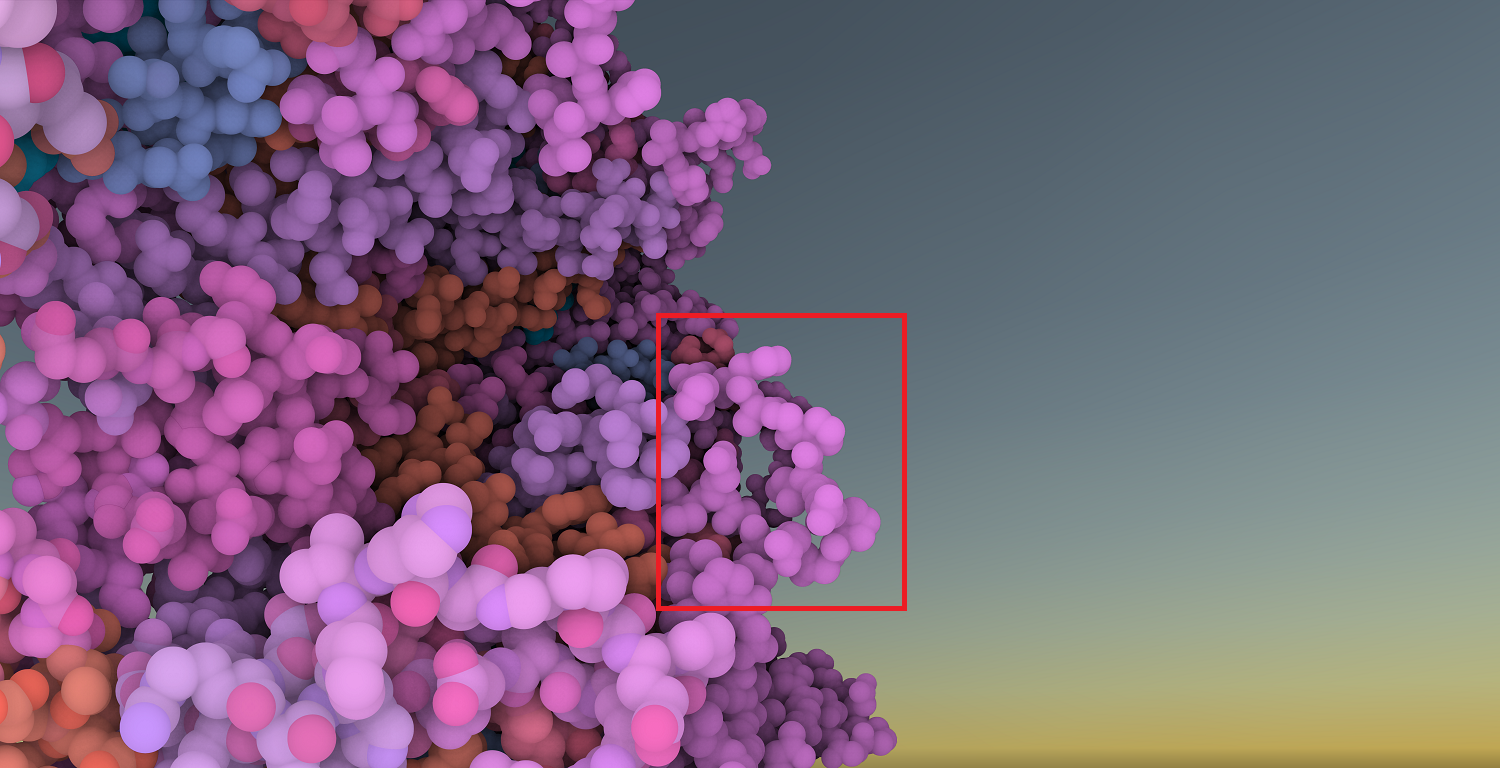
\includegraphics[width=0.95\linewidth,keepaspectratio]{supplementaryMaterial/bindingsite} 
		
		\vspace{0.1cm}
		
		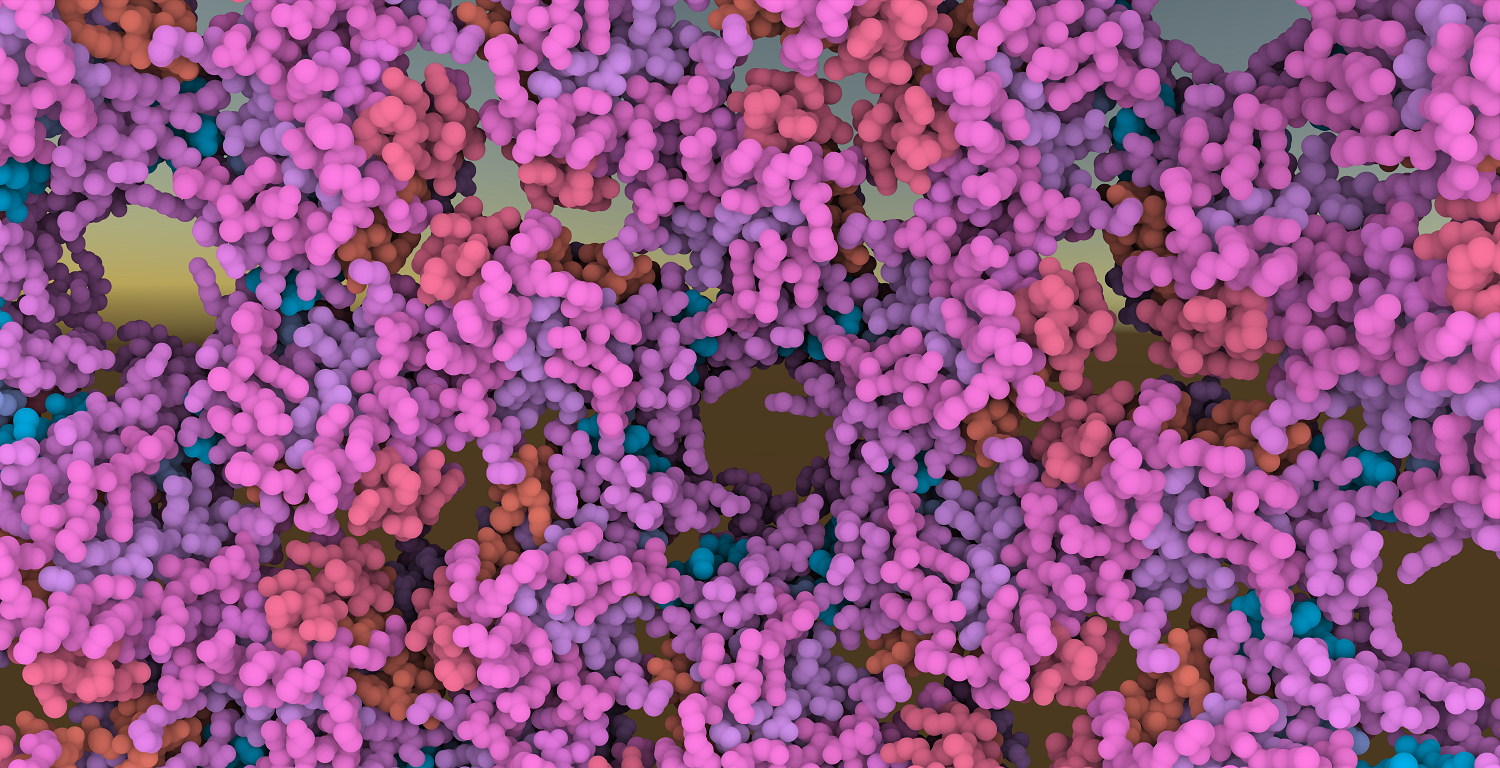
\includegraphics[width=0.95\linewidth,keepaspectratio]{supplementaryMaterial/hexamerhelices} 
		
		\vspace{0.1cm}
		
		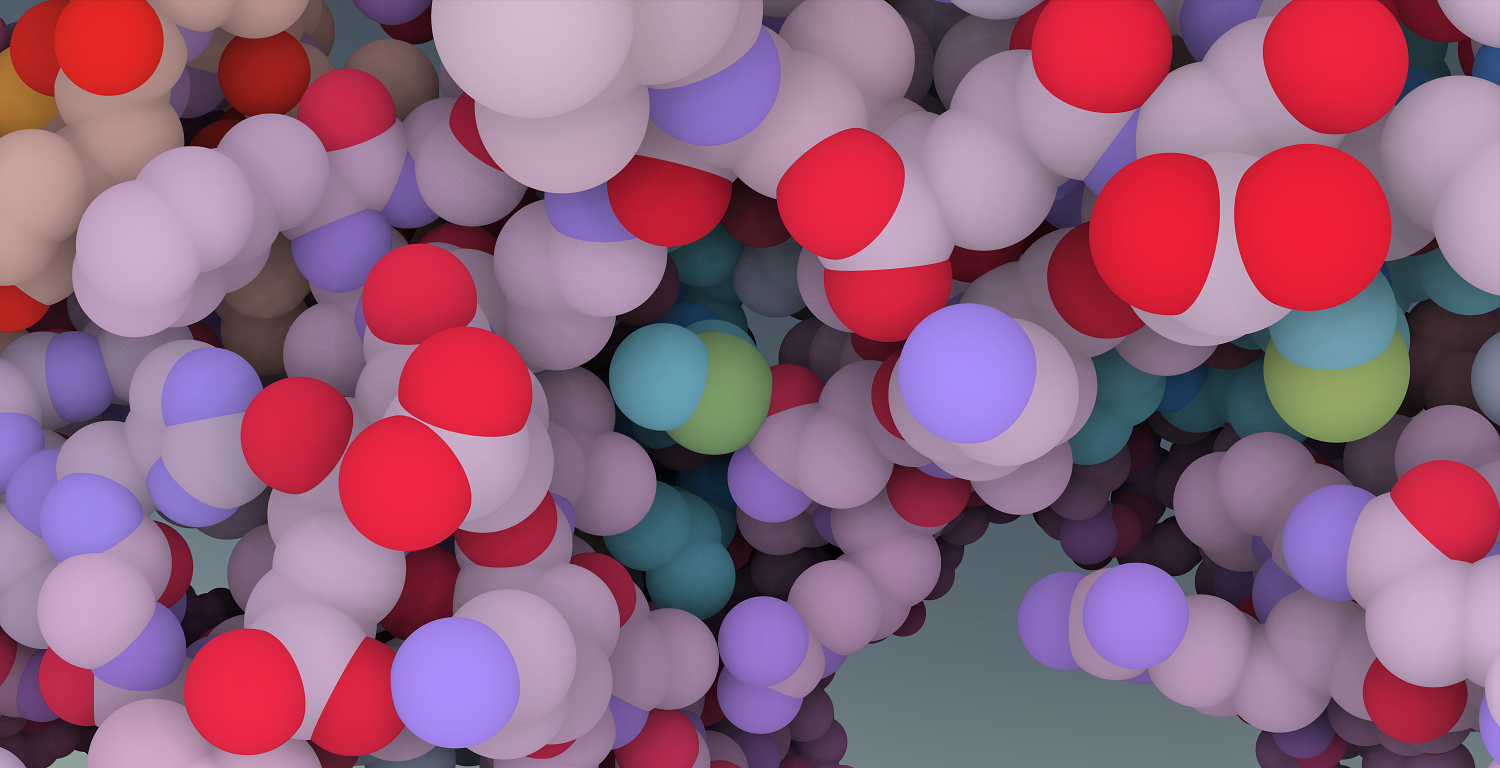
\includegraphics[width=0.95\linewidth,keepaspectratio]{supplementaryMaterial/sulfur} 
		\caption{User study search task. Top: Methionine binding site (red box). Middle: Alpha helices (blue). Bottom: Sulfur (yellow).}
	\end{figure}
	
	
	
	
\end{document}